\documentclass[11pt,a4paper]{article}
\usepackage[utf8]{inputenc}
\usepackage{geometry}
\usepackage{amsmath,amssymb,amsthm,mathtools}
\usepackage{booktabs}
\usepackage{array}
\usepackage{graphicx}
\usepackage{enumitem}
\usepackage{xcolor}
\usepackage{pgfplots}
\usepackage{algorithm}
\usepackage[noend]{algpseudocode}
\usepackage{hyperref}
\pgfplotsset{compat=1.16}
\geometry{left=2.5cm,right=2.5cm,top=2.5cm,bottom=2.5cm}
\hypersetup{colorlinks=true,linkcolor=blue!50!black,citecolor=blue!50!black,urlcolor=blue!55!black,
  pdftitle={Anchored Sparse-Offset Screening of Semiprimes: An Exact Sieve Null Model, Two-Adic Saturation, and Positive-Control Benchmarks up to 2048 Bits},
  pdfauthor={Arsen A. Khachatryan},
  pdfsubject={Preprint, Version 11.0.3},
  pdfkeywords={semiprime; Fermat factorisation; quadratic-residue sieve; weak keys; two-adic saturation; positive controls; reproducible benchmark}}

\newtheorem{definition}{Definition}[section]
\newtheorem{proposition}{Proposition}[section]
\newtheorem{corollary}{Corollary}[section]
\newtheorem{remark}{Remark}[section]
\newcommand{\Z}{\mathbb Z}
\newcommand{\Zp}{\mathbb Z_2}
\newcommand{\code}[1]{\texttt{#1}}
\DeclareMathOperator{\lcm}{lcm}

\title{\textbf{Anchored Sparse-Offset Screening of Semiprimes:\\
An Exact Sieve Null Model, Two-Adic Saturation,\\
and Positive-Control Benchmarks up to 2048 Bits}}
\author{Arsen A. Khachatryan\\
\small SibarS Labs, SibarS Group of Companies, Tallinn, Estonia\\
\small ORCID: 0009-0006-7629-3833 \quad \texttt{cto@sibars.net}}
\date{Preprint, Version 11.0.3 \quad $\cdot$ \quad 4 October 2026\\[2pt]
\small Not peer reviewed. Licence: CC BY-NC 4.0.}

\begin{document}
\maketitle


\begin{abstract}
We study a family of structured semiprimes $n=pq$ for which the weighted arithmetic centre $(ap+bq)/2$ lies in a public \emph{anchored sparse set} $2^r+\mathcal Z$, where $\mathcal Z$ consists of all integers with $h$ binary ones inside a $w$-bit window. Membership is certified by the Lehman--Hart-type identity $A^2-abn=\bigl((ap-bq)/2\bigr)^2$, so the screen is sound by construction. Our contributions are quantitative rather than algebraic. (i)~We prove that for an odd prime $\ell\nmid N$ the fraction of residues $A \bmod \ell$ with $A^2-N$ a square is \emph{exactly} $\tfrac12+\chi_\ell(N)/(2\ell)$, which gives a closed-form null model for a quadratic-residue sieve and a rule (``adaptive primes'') that roughly halves the number of exact tests. (ii)~We prove that two-adic filtering saturates: the pass density modulo $2^m$ is bounded below by a positive constant independent of $m$, so no amount of two-adic lifting can substitute for odd moduli. This explains why the two-adic ``screen'' of an earlier preprint finds only the slice $z=0$. (iii)~We give a lazily generated representation of the offset set that removes the previous limit $w\le 255$ and report benchmarks on planted moduli of 1024 and 2048 bits with up to $3.3\times10^{8}$ offsets ($\kappa=\log_2|\mathcal Z|\approx 28.3$), in which every planted factorisation was recovered, with a single exact square test after sieving once about $1.1\kappa$ primes were used, and with no false positive among random moduli. A pre-specified audit of 2{,}355 public GitHub SSH RSA moduli (about $1.9\times10^{10}$ centre hypotheses in total, one CPU core, 17 minutes) found no modulus in any tested family and no shared prime, while all 88 planted controls were recovered; this is a negative result that validates the pipeline rather than a finding about keys. The method does not threaten properly generated RSA keys; its intended role is as a calibrated positive-control and audit tool for hypothesised generator defects.
\end{abstract}

\noindent\textbf{Keywords:} semiprime; Fermat factorisation; Lehman's method; quadratic-residue sieve; weak keys; two-adic saturation; positive controls; reproducible benchmark

\section{Introduction}
Auditing cryptographic key material for \emph{structured} defects is a different task from factoring generic RSA moduli. Large measurements of deployed keys~\cite{heninger,lenstra,hastings,svenda,nemec} have shown that defects are caused by implementation flaws---low-entropy generators, shared primes, structured prime generation---not by weaknesses of well-generated keys. A practical audit needs (a)~algorithms that are \emph{exact} when a hypothesised defect is present, (b)~a calibrated account of what they cost and how often they err on unstructured data, and (c)~honest statements of what they cannot do.

This paper takes the algebraic idea from the author's preprint cycle~\cite{zenodo10} (centres that are compressible relative to a dyadic anchor) and removes everything that is not needed for it. The underlying identity is classical: if $ap+bq=2A$, then $A^2-abn$ is a perfect square, which is the principle of Fermat's method with the multipliers of Lehman~\cite{lehman} and Hart~\cite{hart} and of the sieving of McKee~\cite{mckee}. We make no claim to that identity. What we add is the following.

\begin{enumerate}[label=\textbf{C\arabic*.},leftmargin=2.2em,itemsep=2pt]
\item \textbf{Unification.} One parametrised family $(r,k,z)$ with $k=ab$ and $z$ in a public sparse set covers both the two-adic ``screen'' of the preprint~\cite{zenodo5} and the centre search of~\cite{zenodo10}; the former is the slice $z=0$ (Section~\ref{sec:v5}).
\item \textbf{Exact sieve null model} (Proposition~\ref{prop:pass}): pass fraction $\tfrac12+\chi_\ell(N)/(2\ell)$, hence an optimal prime-selection rule.
\item \textbf{Two-adic saturation} (Proposition~\ref{prop:sat}): the two-adic part of the sieve contributes at most a constant factor, whatever the number of bits.
\item \textbf{Scalable offset sets.} A lazy generator for $\binom{w}{h}$ offsets with arbitrary $w$; benchmarks on 1024- and 2048-bit planted moduli up to $\kappa\approx 28.3$ (Section~\ref{sec:exp}).
\item \textbf{A pre-specified corpus audit} of 2{,}355 public RSA moduli with planted end-to-end controls (Section~\ref{sec:corpus}); the outcome is negative and is reported as such.
\item \textbf{Reference software} with self-tests, benchmark and audit scripts.
\end{enumerate}

\paragraph{Relation to earlier versions.} This is Version 11.0.3 of a preprint series on dyadic shells in semiprime arithmetic (all versions: Zenodo concept DOI 10.5281/zenodo.20306132; earlier versions~\cite{zenodoseries,zenodo5,zenodo10}). Version 10.5.1~\cite{zenodo10} introduced centre-compressible semiprimes and a $41{,}664$-candidate benchmark; the present version re-derives the screen as a single sound scan over an arbitrary public set of offsets, adds the sieve and saturation results, scales the benchmarks to $\binom{w}{h}\approx3.3\times10^{8}$ offsets and 2048-bit moduli, and reports a corpus audit.

\paragraph{What is not claimed.} No attack on RSA keys generated by a sound procedure; no new factoring algorithm; no evidence that any deployed key population is anchor-compressible.

\section{Related work}
Fermat's method and its multiplier variants are due to Fermat and Kraitchik~\cite{kraitchik}, Lehman~\cite{lehman}, McKee~\cite{mckee} (who studies speed-ups of the square test by sieving), and Hart~\cite{hart}, whose one-line algorithm examines $\lceil\sqrt{kn}\rceil$ for successive $k$. De~Weger~\cite{deweger} shows that the cost of Fermat's method is $O(\Delta^2/\sqrt n)$ for $\Delta=|p-q|$, so that $\Delta<n^{1/4}$ gives an almost instantaneous factorisation, and notes that ANSI X9.31 requires the two primes to differ in their first $100$ bits. Lattice methods of Coppersmith~\cite{copp96b,copp97} recover a factor from about half of its most or least significant bits; Howgrave-Graham~\cite{hg01} places them in the framework of approximate common divisors and shows in particular that $p$ is recovered from any $p_0=kp+x_0$ with $|x_0|<N^{1/4}$ when $p\sim q\sim\sqrt N$.

Such methods have been applied to structured primes in the wild. Bernstein et al.~\cite{bernstein} factored $184$ of more than two million $1024$-bit keys of the Taiwanese Citizen Digital Certificate database, $103$ of them by batch GCD and the rest, after identifying prime factors whose binary expansion repeats a short bit pattern with sporadic errors, by Coppersmith-type attacks. Nitaj and Rachidi~\cite{nitaj} define ``weak primes'' $ap=u_0+M_1u_1+\dots+M_ku_k$ with small parameters and give lattice bounds for factoring; Rivest and Silverman~\cite{rivest} discuss whether ``strong'' primes are needed. Corpus studies of weak keys include batch-GCD surveys~\cite{heninger,lenstra,hastings,barbulescu}---Barbulescu et al.~\cite{barbulescu} also crawled public GitHub SSH keys through the endpoint used in Section~\ref{sec:corpus}---, attribution of keys to their software origin from biases of the public modulus~\cite{svenda}, and the detection of the ROCA structure~\cite{nemec}. Our audit statistic is related to the last two but differs in kind: it is an arithmetic test (a square test on a hypothesised set of centres) rather than a statistical fingerprint of the generator. Moreover, the defects observed so far concern prime factors (shared primes, patterned primes), whereas the hypothesised structure here concerns the centre $(p+q)/2$.

\section{Framework}\label{sec:framework}
Throughout, $n=pq$ with distinct odd primes $p,q$.

\begin{definition}[Anchored sparse family]
Fix integers $1\le h\le w\le r$. Let
\[
\mathcal Z(w,h)=\Bigl\{\textstyle\sum_{i=1}^h 2^{e_i}\;:\;0\le e_1<\dots<e_h<w\Bigr\},\qquad |\mathcal Z(w,h)|=\binom wh,\qquad \kappa=\log_2|\mathcal Z|.
\]
The \emph{anchored centre set} is $2^r+\mathcal Z(w,h)$; $\kappa$ is its search entropy. A contiguous window $\{z:|z|<2^{\zeta}\}$ is a second admissible choice of $\mathcal Z$.
\end{definition}

\begin{definition}[Compressibility]
$n$ is \emph{$(K,\mathcal Z,r)$-compressible} if for some coprime odd integers $a,b$ with $ab\in K$, $1\le a,b<\min(p,q)$, and some $z\in\mathcal Z$: $ap+bq=2(2^r+z)$ (after possibly swapping $p,q$).
\end{definition}

\begin{remark}[Parity]\label{rem:parity}
Since $p,q$ are odd, $ap+bq$ is even iff $a+b$ is even; with $\gcd(a,b)=1$ this forces $a,b$ odd, so \emph{only odd $k=ab$ occur}. The implementation scans all $k\le k_{\max}$, so restricting to odd $k$ would halve the work (not implemented).
\end{remark}

\begin{proposition}[Soundness and recovery]\label{prop:rec}
Let $A\in\Z$ and $a,b$ be as above with $ap+bq=2A$. Then $A^2-abn=t^2$ with $t=(ap-bq)/2\in\Z$, and $\{\gcd(A-t,n),\gcd(A+t,n)\}=\{q,p\}$ up to order. Conversely, for any $A,k,t$ with $A^2-kn=t^2$ every $d\in\{\gcd(A\pm t,n)\}$ with $1<d<n$ is a proper divisor of $n$.
\end{proposition}
\begin{proof}
$ap\equiv bq \pmod 2$, so $t\in\Z$; $A+t=ap$ and $A-t=bq$, hence $A^2-t^2=abpq$. As $a<q$ and $b<p$ are not multiples of the respective primes, $\gcd(ap,pq)=p\gcd(a,q)=p$ and $\gcd(bq,pq)=q$. For the converse, $d\mid n$ by definition.
\end{proof}
\begin{remark}[Fermat's axis]\label{rem:fermat}
De~Weger's lemma~\cite{deweger} states that for $\Delta=q-p$ one has $0<p+q-2\sqrt n<\Delta^2/(4\sqrt n)$, i.e.\ $0<A-\sqrt n<\Delta^2/(8\sqrt n)$. A Fermat search started at $\lceil\sqrt n\rceil$ therefore needs about $\Delta^2/(8\sqrt n)$ steps, whereas an anchored search costs $|\mathcal Z|$ steps irrespective of $\Delta$: closeness of the primes and compressibility of the centre are independent parameters.
\end{remark}
The case $k=1$, $z=0$ reads $n=2^{2r}-t^2$ (a ``dyadic shell''); $k=1$ is Fermat's method started at a hypothesised centre; $k>1$ is the identity $x^2-4kn=y^2$ of Lehman and Hart with $x=2A$.

\section{Sieve theory}\label{sec:sieve}
For a candidate centre $A$ the number $A^2-kn$ can be a perfect square only if it is a square modulo every modulus $m$. Write $N=kn$.

\begin{proposition}[Exact pass fraction]\label{prop:pass}
Let $\ell$ be an odd prime with $\ell\nmid N$ and $\chi$ the Legendre symbol. The number of residues $A\bmod\ell$ for which $A^2-N$ is a square (or zero) modulo $\ell$ equals $(\ell+\chi(N))/2$, i.e. the pass fraction is
\[
f_\ell(N)=\frac12+\frac{\chi(N)}{2\ell}.
\]
\end{proposition}
\begin{proof}
Count pairs $(A,y)\in\mathbb F_\ell^2$ with $A^2-y^2=N$. With $u=A-y$, $v=A+y$ (a bijection since $2$ is invertible) the equation is $uv=N$, which has $\ell-1$ solutions. For each $A$ the number of $y$ is $1+\chi(A^2-N)$ (with $\chi(0)=0$). Let $N_0=\#\{A:A^2=N\}=1+\chi(N)$ and $N_{\square}$ the number of $A$ with $A^2-N$ a non-zero square. Then $2N_\square+N_0=\ell-1$, so $N_\square=(\ell-2-\chi(N))/2$, and the number of passing residues is $N_\square+N_0=(\ell+\chi(N))/2$.
\end{proof}
We verified the count numerically for $11{,}568$ pairs $(N,\ell)$ ($300$ random $N$, the $40$ smallest odd primes) with no mismatch.

\begin{corollary}[Null model and prime selection]\label{cor:null}
If the $M$ candidate residues are equidistributed modulo each chosen $\ell_1,\dots,\ell_j$ and independent across them, a random $n$ leaves $M\prod_{i}f_{\ell_i}(kn)$ false survivors. For fixed $j$ the product is minimised by taking the $j$ primes with smallest $f_\ell$, i.e.\ first those with $\chi_\ell(kn)=-1$ (``adaptive primes''). For $\ell=3$ the choice changes the pass fraction from $2/3$ to $1/3$.
\end{corollary}
Equidistribution is a heuristic for sparse sets, supported but not proved here (Section~\ref{sec:exp}).

\begin{proposition}[Two-adic saturation]\label{prop:sat}
Let $N\ge3$ be odd and $\pi_m(N)$ the proportion of residues $A\bmod 2^m$ for which $A^2-N$ is a square modulo $2^m$. Then $\pi_m$ is non-increasing and $\pi_m(N)\ge 2^{-(2v+3)}>0$ for every $m$, where $v=v_2\bigl((N-1)/2\bigr)$. In particular a two-adic prefilter, however many bits it uses, reduces the number of (equidistributed) candidates by at most a constant factor independent of $m$.
\end{proposition}
\begin{proof}
Squareness modulo $2^{m+1}$ implies squareness modulo $2^m$, so $\pi_m$ is non-increasing. Put $A_0=(N+1)/2$; then $A_0^2-N=u^2$ with $u=(N-1)/2\neq0$, $u=2^vw$, $w$ odd. If $A\equiv A_0\pmod{2^{2v+3}}$ then $A^2-N\equiv u^2\pmod{2^{2v+3}}$, i.e.\ $A^2-N=2^{2v}(w^2+8s)$ for some $s\in\Zp$, and $w^2+8s\equiv1\pmod 8$ is a square in $\Zp$ by Hensel's lemma. Hence all such $A$ have $A^2-N$ a 2-adic square, hence a square modulo every $2^m$. These $A$ form a set of density $2^{-(2v+3)}$.
\end{proof}
Numerically (Table~\ref{tab:twoadic}) the limit depends only on $N\bmod8$: $1/4$ for $N\equiv3,7$, $1/8$ for $N\equiv5$, and for $N\equiv1$ a slow decrease to about $1/24$ ($0.04175$ at $m=16$; the value $1/24$ is conjectural). Each odd prime, by contrast, contributes a factor near $1/2$ which multiplies.

\begin{table}[ht]\centering\small
\caption{Fraction of $A \bmod 2^m$ with $A^2-N$ a square modulo $2^m$ (computed exhaustively).}\label{tab:twoadic}
\begin{tabular}{@{}rrrrrr@{}}\toprule
$N \bmod 8$ & $m=4$ & $m=6$ & $m=8$ & $m=12$ & $m=16$\\\midrule
3 or 7 & 0.25 & 0.25 & 0.25 & 0.25 & 0.25\\
5 & 0.25 & 0.125 & 0.125 & 0.125 & 0.125\\
1 & 0.25 & 0.125 & 0.0625 & 0.04297 & 0.04175\\\bottomrule
\end{tabular}
\end{table}

\begin{remark}[Sparse sets act as a two-adic gate]
For $\mathcal Z(w,h)$ the proportion of offsets with all exponents $\ge m$, namely $\binom{w-m}{h}/\binom wh$, tends to $1$ as $w\to\infty$; for $m=6$, $w=64$, $h=3$ it is $74\%$. Almost all candidates then satisfy $A\equiv 2^r\equiv0 \pmod{2^m}$, so the table modulo $2^m$ does not thin the set gradually: it removes nearly all of it unless $-N$ is a square modulo $2^m$ (an event of probability about $1/4$ to $1/8$ for random $n$), and in that case it keeps nearly all. For a planted modulus the gate always opens, because the true centre passes. This makes the number of exact tests heavy-tailed over random $n$.
\end{remark}

\section{Algorithm and cost}\label{sec:alg}
\begin{algorithm}[ht]
\caption{$(k,z)$-scan with adaptive sieve}\label{alg:scan}
\begin{algorithmic}[1]
\Require odd $n$; anchors $R$; weights $K$; offset set $\mathcal Z$ (lazily generated); $j$ odd primes
\For{$r\in R$, $k\in K$}
  \State $N\gets kn$; choose primes $\ell_1,\dots,\ell_j\nmid N$ with smallest $f_\ell(N)$ (Proposition~\ref{prop:pass})
  \State precompute tables $T_m[a]=[\,a^2-N \text{ is a square mod } m\,]$ for $m\in\{64,\ell_1,\dots,\ell_j\}$
  \For{each block of offsets $\mathcal B\subset\mathcal Z$}
    \State compute $z\bmod m$ for the surviving $z\in\mathcal B$ and keep those with $T_m[(2^r+z)\bmod m]=1$, in the order $64,\ell_1,\dots$
    \For{each survivor $z$}
      \State $A\gets 2^r+z$; $D\gets A^2-N$; \textbf{if} $D\ge0$ and $\lfloor\sqrt D\rfloor^2=D$ \textbf{then} $t\gets\lfloor\sqrt D\rfloor$
      \State \textbf{output} every $d\in\{\gcd(A\pm t,n)\}$ with $1<d<n$
    \EndFor
  \EndFor
\EndFor
\end{algorithmic}
\end{algorithm}
\paragraph{Cost.} The sieve costs $O(1)$ word operations per candidate until it terminates, and each exact test costs one big-integer multiplication and square root. By Corollary~\ref{cor:null}, a scan of $M=|\mathcal Z|$ offsets performs about $1+M\prod f_{\ell_i}$ exact tests, so about $j\approx\kappa/\log_2(1/\bar f)$ primes are needed with $\bar f\approx 0.48$. Memory is $O(\text{block}+\text{tail table})$. Besides the anchor $2^r$ the implementation accepts both signs ($A=2^r\pm z$, needed for centres just below a power of two) and an arbitrary integer base such as $\lceil\sqrt n\rceil$, which turns the same code into a sieved Fermat search. The implementation (Python/NumPy) examines about $6\times10^{6}$ offsets per second per core in our runs.

\section{Relation to the two-adic ``screen'' of the preprint cycle}\label{sec:v5}
The preprint~\cite{zenodo5} looks for triples $(r,s,\alpha)$ with $2^{2r}-s^2=\alpha n$ by factoring $F=2^{x}-n$ ($x=2r$) with a bounded budget, building square roots modulo $2^x$ and testing the interval condition $\alpha\le\lfloor(2^x-1)/n\rfloor$. For the experiments below the screen was re-implemented from the algorithm description in Sections~18--23 and Remark~21.18 of that preprint.

\begin{proposition}[The congruence alone carries no information]
For odd $\alpha$ with $-\alpha n\equiv1\pmod 8$ and $x\ge3$, the congruence $s^2\equiv-\alpha n\pmod{2^x}$ has exactly four solutions modulo $2^x$.
\end{proposition}
Hence for every admissible $\alpha$ a ``two-adically valid'' $s$ exists; the only information about $n$ enters through the interval constraint, which a generic $\alpha$ meets with probability about $1/n$. Consistently, the reconstruction found no exact triple among about $2\times10^5$ candidates for $60$ random semiprimes of each of $24$, $32$ and $40$ bits. A non-trivial triple is a mixed square root of $2^{2r}$ modulo $n$, so finding one is as hard as factoring $n$.

What the screen can detect is the slice $z=0$. Table~\ref{tab:v5} compares it with Algorithm~\ref{alg:scan} on planted $48$-bit moduli. The new scan covers all rows, in about a quarter of the time. (The old screen does not scale: for $128$ bits it must factor an integer of about $256$ bits; we did not attempt this.)

\begin{table}[ht]\centering\small
\caption{Planted 48-bit moduli, 6 instances per row: $ap+bq=2(2^{24}+z)$. Success = non-trivial factor found. Scan: window $|z|<2^{13}$, $k\le30$, 3 anchors.}\label{tab:v5}
\begin{tabular}{@{}lrrrr@{}}\toprule
$(a,b,z)$ & preprint screen & $(k,z)$-scan & screen time (s) & scan time (s)\\\midrule
$(1,1,0)$ & 6/6 & 6/6 & 0.47 & 0.11\\
$(1,1,5)$ & 0/6 & 6/6 & 0.63 & 0.11\\
$(1,1,-3000)$ & 0/6 & 6/6 & 0.38 & 0.12\\
$(1,3,0)$ & 6/6 & 6/6 & 0.33 & 0.11\\
$(3,5,1233)$ & 0/6 & 6/6 & 0.34 & 0.11\\
$(3,5,-777)$ & 0/6 & 6/6 & 0.17 & 0.11\\\bottomrule
\end{tabular}
\end{table}

\section{Experiments}\label{sec:exp}
\paragraph{Setup.} \code{dyadic\_kz\_scan.py} (Python~3, NumPy; \code{gmpy2} only for generating test moduli). Positive controls are planted: pick $z$ at random in $\mathcal Z(w,h)$, a prime $p$ of $r$ bits, and require $q=2(2^r+z)-p$ to be prime (so $k=1$; the weighted case is covered by the self-test). Negative controls are products of two random primes of equal length. All runs are single-threaded on one CPU core of a general-purpose virtual machine (CPU model not recorded), with CPython~3, NumPy and, for generating test moduli only, \code{gmpy2}.

\paragraph{E1: null model.} On $N=300$ random $128$-bit moduli with $\mathcal Z(64,3)$ ($41{,}664$ offsets), the $64$-table and $12$ odd primes, the observed number of survivors reaching the exact test, relative to the prediction of Corollary~\ref{cor:null} (taking the observed output of the $2$-adic gate as input), was $0.994$ and $1.034$ (plain primes) and $1.032$ and $0.906$ (adaptive primes) in two independent runs (observed totals $859/864$, $715/692$, $430/417$, $320/353$). With $N=20$ the ratio was $0.77$, which shows that the estimator is noisy because of the gate. Adaptive primes reduced the totals by factors $2.0$ and $2.2$. The null model is thus consistent with the data at the $\pm10\%$ level we can resolve; a tighter test needs more samples.

\paragraph{E2: scaling at 1024 bits.} Planted centre $2^{512}+z$, $k=1$, $14$ odd primes (Table~\ref{tab:scaling}).
\begin{table}[ht]\centering\small
\caption{1024-bit planted moduli, $r=512$, one instance per row.}\label{tab:scaling}
\begin{tabular}{@{}rrrrrrr@{}}\toprule
$w$ & $h$ & $|\mathcal Z|$ & $\kappa$ & scan (s) & exact tests & found\\\midrule
64 & 3 & 41,664 & 15.35 & $<0.1$ & 1 & yes\\
128 & 3 & 341,376 & 18.38 & 0.1 & 11 & yes\\
64 & 4 & 635,376 & 19.28 & 0.1 & 13 & yes\\
96 & 4 & 3,321,960 & 21.66 & 0.5 & 81 & yes\\
128 & 4 & 10,668,000 & 23.35 & 1.7 & 245 & yes\\\bottomrule
\end{tabular}
\end{table}
The last row has the parameters of the 1024-bit certificate of~\cite{zenodo10}. Over $14$ planted instances with $\mathcal Z(128,4)$ all were recovered, with a mean of $332$ exact tests (median $344$, maximum $441$). On $12$ random $1024$-bit semiprimes there was no false positive; the number of exact tests was heavy-tailed (mean $17.2$, median $4$, maximum $164$), as predicted by the gate remark.

\paragraph{E3: number of sieve primes.} For $|\mathcal Z|=10{,}668{,}000$ ($\kappa=23.35$) and $8$ planted instances (Figure~\ref{fig:primes}) the mean number of exact tests was $12{,}351$ (8 primes), $182$ (14), $3.8$ (20), $1.0$ (26) and $1.0$ (32); all $8$ were recovered every time. About $1.1\kappa$ primes therefore suffice to leave only the true centre.

\begin{figure}[ht]\centering
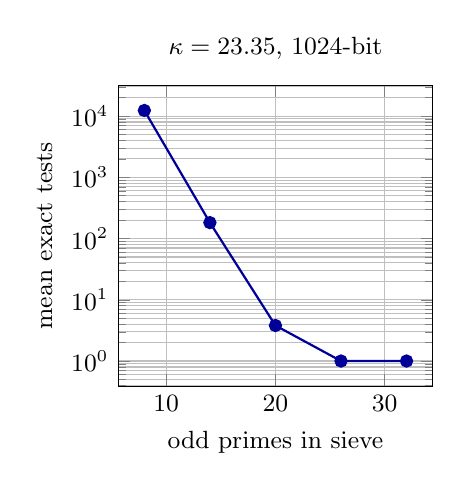
\begin{tikzpicture}
\begin{axis}[width=0.46\textwidth,height=5.4cm,ymode=log,xlabel={odd primes in sieve},ylabel={mean exact tests},grid=both,
  title={\small $\kappa=23.35$, 1024-bit},tick label style={font=\small},label style={font=\small}]
\addplot[mark=*,thick,blue!60!black] coordinates {(8,12351.1) (14,182.1) (20,3.8) (26,1.0) (32,1.0)};
\end{axis}
\end{tikzpicture}\hfill
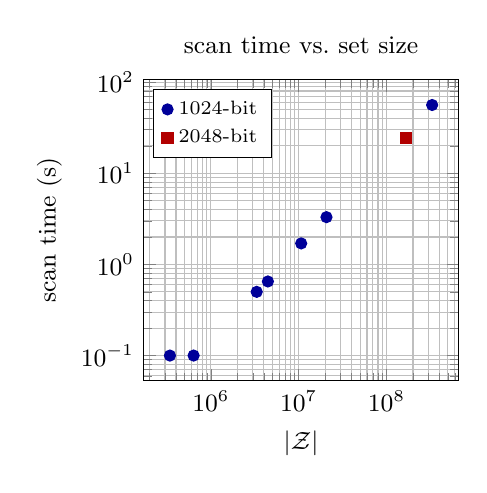
\begin{tikzpicture}
\begin{axis}[width=0.46\textwidth,height=5.4cm,xmode=log,ymode=log,xlabel={$|\mathcal Z|$},ylabel={scan time (s)},grid=both,
  title={\small scan time vs.\ set size},tick label style={font=\small},label style={font=\small},legend pos=north west,legend style={font=\scriptsize}]
\addplot[only marks,mark=*,blue!60!black] coordinates {(341376,0.1) (635376,0.1) (3321960,0.5) (10668000,1.7) (4455100,0.65) (20708500,3.3) (330791175,56.1)};
\addplot[only marks,mark=square*,red!70!black] coordinates {(166167000,24.2)};
\legend{1024-bit,2048-bit}
\end{axis}
\end{tikzpicture}
\caption{Left: exact tests after sieving. Right: scan time grows linearly in $|\mathcal Z|$ (about $6\times10^{6}$ offsets/s). Times in the last rows of Tables~\ref{tab:scaling}--\ref{tab:bigw}.}\label{fig:primes}
\end{figure}

\paragraph{E4: windows wider than 255 bits.} The offset set is generated lazily in blocks (Section~\ref{sec:alg}); it replaces an earlier dense array of exponents that limited $w$ to $255$ and the sizes to a few $10^7$. Table~\ref{tab:bigw} reports planted instances, each recovered with one exact test.
\begin{table}[ht]\centering\small
\caption{Windows wider than 255 bits (number of sieve primes about $1.5\kappa$, not tuned).}\label{tab:bigw}
\begin{tabular}{@{}rrrrrrrr@{}}\toprule
$n$ (bits) & $r$ & $w$ & $h$ & $|\mathcal Z|$ & $\kappa$ & primes & scan (s)\\\midrule
1024 & 512 & 300 & 3 & 4,455,100 & 22.09 & 34 & 0.7\\
1024 & 512 & 500 & 3 & 20,708,500 & 24.30 & 36 & 3.3\\
1024 & 512 & 300 & 4 & 330,791,175 & 28.30 & 42 & 56.1\\
2047 & 1024 & 1000 & 3 & 166,167,000 & 27.31 & 44 & 24.2\\\bottomrule
\end{tabular}
\end{table}
The generator was checked against the dense enumeration on five small $(w,h)$ with different block sizes (identical sets).

\paragraph{E5: misspecified hypotheses.} For planted $\mathcal Z(128,4)$ centres, scanning $\mathcal Z(128,3)$ or $\mathcal Z(64,4)$ recovered $0/6$ and $0/6$. The scan is blind outside the hypothesised family.


\section{Corpus audit}\label{sec:corpus}
\paragraph{Purpose.} The question is not whether planted keys are found (they are, by construction) but whether any \emph{real} key lies in the families of Section~\ref{sec:framework}, and what the audit costs at corpus scale. The answer reported here is negative.

\paragraph{Data.} Public SSH keys published by GitHub users (\code{https://github.com/<user>.keys}); usernames were obtained from the follower pages of 21 large accounts. Two crawls processed $17{,}792$ users (the second crawl examined a random subset of $4{,}000$ of the $29{,}253$ usernames it had collected), of whom $6{,}121$ had at least one published key; $2{,}379$ were \texttt{ssh-rsa} keys, of which $24$ were duplicates (the same account reached by both crawls; no modulus occurs under two different accounts). The remaining \textbf{2,355 distinct moduli} form the corpus; none is shared by two accounts. Key sizes: $3072$ bits $1{,}025$ ($43.5\%$), $4096$ bits $985$ ($41.8\%$), $2048$ bits $327$ ($13.9\%$), and $18$ others ($1024$: $5$, $8192$: $5$, non-standard lengths such as $4068$, $4069$, $4097$). The corpus is a convenience sample of developers who publish keys on a code-hosting service; it is not representative of any deployed population, and it contains no TLS or embedded-device keys, where historical defects were found~\cite{heninger,lenstra,hastings,bernstein}. A crawl of the same endpoint in 2015--2016 reported a very different size distribution (mostly $2048$-bit keys)~\cite{barbulescu}, which reflects the evolution of default key sizes.

\paragraph{Pre-specified battery.} The following four members were fixed after the synthetic tests of Sections~\ref{sec:sieve}--\ref{sec:exp} and before any real key was scanned; they were not modified afterwards. For each modulus $n$ of $L$ bits, $r_{\min}=\lceil L/2\rceil$ and, for weight $k$, $r_k=\lceil \mathrm{bitlen}(kn)/2\rceil$. All use $24$ adaptively chosen odd primes.
\begin{enumerate}[leftmargin=1.8em,itemsep=1pt]
\item[\textbf{W}] contiguous window $|z|<2^{16}$, odd $k\in\{1,3,\dots,15\}$, anchors $r_k,r_k+1,r_k+2$ ($3.15\times10^6$ hypotheses);
\item[\textbf{S3}] $\mathcal Z(128,3)$ with $A=2^r\pm z$, $k=1$, $r\in\{r_{\min},r_{\min}+1\}$ ($1.37\times10^6$);
\item[\textbf{S4}] $\mathcal Z(64,4)$, same signs and anchors ($2.54\times10^6$);
\item[\textbf{F}] a Fermat baseline $A=\lceil\sqrt n\rceil+z$, $0\le z<2^{20}$ ($1.05\times10^6$).
\end{enumerate}
Altogether $8{,}101{,}312$ centre hypotheses per modulus. As a second, independent check we ran a batch GCD over the corpus (shared prime factors).

\paragraph{Controls.} Mixed into the same run, in random order and through the identical code path, were $88$ planted moduli: $22$ for each of W, S3, S4 and F ($16$ of $1024$ and $6$ of $2048$ bits each), generated as in Section~\ref{sec:exp}.

\begin{table}[ht]\centering\small
\caption{Corpus audit. Controls are detected only by the battery member that matches their construction.}\label{tab:corpus}
\begin{tabular}{@{}lr@{}}\toprule
Distinct RSA moduli audited & 2,355\\
Shared prime factors (batch GCD) & 0\\
Hypotheses tested per modulus & 8,101,312\\
Hypotheses tested in total & $1.908\times10^{10}$\\
Exact square tests performed (real keys) & 128 ($0.054$ per key)\\
\textbf{Real moduli in any family (W, S3, S4, F)} & \textbf{0}\\
Planted controls detected & 88/88\\
\quad W / S3 / S4 / F & 22/22 each\\
Time (single CPU core, CPython) & 1,000 s ($\approx0.4$ s per modulus)\\\bottomrule
\end{tabular}
\end{table}

\paragraph{Results.} (i)~No real modulus lies in any of the four families, and the batch GCD finds no shared prime. (ii)~All $88$ controls were recovered, and each by exactly the intended member; there were no certified false positives, which is expected since every report is verified by $n\bmod d=0$. (iii)~The $128$ exact square tests on real keys, all negative, are of the order the null model predicts: on a random subsample of $400$ real moduli, the sieve left $4$ survivors for $\mathcal Z(64,4)$ (predicted $2.0$) and $0$ for $\mathcal Z(128,3)$ (predicted $1.1$) for one anchor and sign, consistent with Corollary~\ref{cor:null} within Poisson noise. The counts are too small to test the model further on real data. (iv)~The audit runs at roughly $0.06$ s (W), $0.10$ s (S3), $0.23$ s (S4) and $0.02$ s (F) per modulus.

\paragraph{Interpretation.} Several widely used libraries fix the two most significant bits of each prime to $11_2$~\cite{svenda}. Under the model of independent primes uniform on $[3\cdot2^{k-1},2^k)$, $k=L/2$ (up to prime-density factors), the centre $A=(p+q)/2$ has a triangular density on that interval: any fixed set of $M$ values has probability of order $M\,2^{-k}$, and a window of half-width $2^w$ just below $2^k$ has probability about $2^{2(w-k)+3}$. Both are negligible for the hypotheses of the battery ($M\approx8\times10^{6}$, $k\ge512$); a hit would therefore have been a certificate of a generation defect, not a statistical fluctuation. The absence of hits says only that none of $2{,}355$ keys, which are predominantly of the $3072$- and $4096$-bit sizes typical of recent practice (the generating software was not identified), lies in these families. A rule-of-three bound ($3/2355\approx0.13\%$ at $95\%$) would apply only if the sample were random from a population, which it is not; we do not draw a population-level conclusion. The result is useful for three reasons: it shows that the pipeline produces no false alarms on real data, it measures the cost of testing $8\times10^{6}$ hypotheses per key at corpus scale, and it supplies a baseline against which the same battery can be run on corpora where defects are known to exist.

\paragraph{Ethics and disclosure.} Only public keys were read; no username, e-mail address or other personal datum was stored or is reported (keys were kept under a salted hash of the account name, which is not published). Follower pages were fetched sequentially with a pause of $0.4$ s, key files with $8$ concurrent connections, and HTTP~429 responses triggered back-off; the crawler's contact address was sent in the request header. Had a key been flagged, it would have been checked arithmetically and reported privately to its owner, not published.

\paragraph{Limitations of the audit.} (i)~Convenience sample of one platform and one key type. (ii)~Controls were planted at $1024$ and $2048$ bits only, whereas $85\%$ of the corpus uses $3072$ or $4096$; the sieve is size-independent, but the claim ``controls recovered'' is therefore not directly tested at those lengths (Table~\ref{tab:bigw} covers $2047$ bits). (iii)~The families were chosen by the author on the basis of the preprint cycle, so the audit tests those hypotheses only. (iv)~Timings come from one core of a virtual machine whose CPU model was not recorded.

\section{Discussion and limitations}
\paragraph{Nature of the contribution.} Everything algebraic is classical (Proposition~\ref{prop:rec}); the new material is the exact null model (Proposition~\ref{prop:pass}, itself an elementary counting argument that is probably known to implementers of Fermat sieves), the saturation statement (Proposition~\ref{prop:sat}), the scalable offset representation, and the measurements. The corpus audit of Section~\ref{sec:corpus} is negative, so the value of the paper remains methodological: an exact, calibrated and cheap screen with measured costs, not a finding about keys.

\paragraph{Positive controls are planted.} Recovery rates of $100\%$ are consequences of the construction. What the experiments test is correctness of the software, the validity of the sieve model, the cost curve and, in Section~\ref{sec:corpus}, the absence of false alarms on real moduli.

\paragraph{Comparison with lattice methods.} A centre known up to an error $z$ yields an approximation of a prime factor. With $A'=2^r$ and $p'=A'-\sqrt{A'^2-n}$, the derivative of $A\mapsto A-\sqrt{A^2-n}$ at the true centre equals $-p/B$ with $B=(q-p)/2$, so to first order $|p-p'|\approx|z|\,p/B$. For balanced primes $p/B$ is a modest constant unless $q-p$ is small, in which case Fermat's method already applies~\cite{deweger}. Since $p$ is recovered in polynomial time from an approximation with error below about $n^{1/4}$~\cite{copp96b,hg01}, a window of $w\lesssim\tfrac14\log_2 n$ bits is, to this order, within reach of lattice reduction without any search. In Tables~\ref{tab:scaling}--\ref{tab:bigw} this concerns the rows with $w\le128$ at $1024$ bits ($n^{1/4}=2^{256}$); the rows with $w=300$ and $w=500$ at $1024$ bits and $w=1000$ at $2048$ bits ($n^{1/4}=2^{512}$) lie outside that range, where the sparsity of $\mathcal Z$ is what makes a scan feasible. We did not run a lattice implementation, so this comparison rests on the cited bounds and the first-order calculation, not on measurements; hybrid strategies (enumerate the leading exponents, solve the remainder by lattice reduction) are an obvious variant that we have not analysed.

\paragraph{Patterned primes.} The defects that have actually been observed concern prime factors: shared primes~\cite{heninger,lenstra} and primes with a repeating bit pattern~\cite{bernstein}. Testing divisibility of a modulus by a family of patterned primes is a natural companion to the centre-based battery used here and is left for future work.

\paragraph{Other limitations.} (i)~Independence across moduli is a heuristic. (ii)~Timings come from one core of a virtual machine with an unrecorded CPU model and an interpreted language. (iii)~Sample sizes in E1--E5 are small. (iv)~Only odd $k$ can occur (Remark~\ref{rem:parity}); the code scans all.

\section{Conclusions and achievements}
We reduced the author's two earlier search procedures to one sound parametrised scan, proved an exact pass fraction for the quadratic-residue sieve (and thereby an optimal prime-selection rule that halves the number of exact tests in our runs), proved that two-adic filtering saturates (which formalises why the two-adic screen of the preprint cycle cannot be strengthened by lifting), extended the scan to offset sets of arbitrary span, and showed on planted 1024- and 2048-bit moduli with up to $3.3\times10^{8}$ offsets that the cost grows linearly in $|\mathcal Z|$ with essentially one exact test after sieving. A pre-specified audit of $2{,}355$ public RSA moduli ($1.9\times10^{10}$ hypotheses, 17 minutes on one core) found no key in any tested family and recovered all 88 planted controls; it is a negative result that validates the pipeline. The principal open items are audits on corpora where defects are known to occur (TLS, embedded devices), a head-to-head experimental comparison with lattice methods, and tests of patterned primes; until then the work is a methodology, not yet a finding.

\section*{Data and code availability}
The software (\code{dyadic\_kz\_scan.py}, \code{dyadic\_kz\_bench.py}, \code{corpus\_collect.py}, \code{corpus\_audit.py}), a README and the aggregate outcome of the corpus audit (\code{corpus\_audit\_results.json}) are archived together with this preprint on Zenodo. \code{dyadic\_kz\_scan.py --selftest} checks the scan; \code{dyadic\_kz\_bench.py} (\code{nullmodel}, \code{scaling}, \code{primes}, \code{bigw}, \code{twoadic}) regenerates Tables~\ref{tab:twoadic}--\ref{tab:bigw} up to statistical variation. The key corpus itself is not redistributed; the aggregate results contain no keys and no account names.

\section*{Declarations}
\paragraph{Use of generative AI.} During preparation of this manuscript, the author used generative AI tools for drafting assistance, language editing, code review, and organization of numerical experiments. The author reviewed and edited all AI-assisted outputs, independently checked the mathematical statements, computations, benchmark results, citations, and interpretations, and takes full responsibility for the submitted manuscript.
\paragraph{Funding.} This research received no external funding.
\paragraph{Competing interests.} The author declares no conflict of interest.

\begin{thebibliography}{99}\small
\bibitem{lehman} R.~S. Lehman, Factoring large integers, \emph{Math.\ Comp.} 28 (1974), 637--646. doi:10.1090/S0025-5718-1974-0340163-2.
\bibitem{mckee} J.~McKee, Speeding Fermat's factoring method, \emph{Math.\ Comp.} 68 (1999), 1729--1737. doi:10.1090/S0025-5718-99-01133-3.
\bibitem{hart} W.~B. Hart, A one line factoring algorithm, \emph{J.\ Aust.\ Math.\ Soc.} 92 (2012), 61--69. doi:10.1017/S1446788712000146.
\bibitem{deweger} B.~de Weger, Cryptanalysis of RSA with small prime difference, \emph{Appl.\ Algebra Engrg.\ Comm.\ Comput.} 13 (2002), 17--28.
\bibitem{kraitchik} M.~Kraitchik, \emph{Th\'eorie des Nombres}, vol.~II, Gauthier-Villars, Paris, 1926.
\bibitem{copp96} D.~Coppersmith, Finding a small root of a univariate modular equation, in \emph{EUROCRYPT 1996}, LNCS 1070, Springer, 155--165.
\bibitem{copp96b} D.~Coppersmith, Finding a small root of a bivariate integer equation; factoring with high bits known, in \emph{EUROCRYPT 1996}, LNCS 1070, Springer, 178--189.
\bibitem{copp97} D.~Coppersmith, Small solutions to polynomial equations, and low exponent RSA vulnerabilities, \emph{J.\ Cryptology} 10(4) (1997), 233--260.
\bibitem{hg01} N.~Howgrave-Graham, Approximate integer common divisors, in \emph{Cryptography and Lattices (CaLC 2001)}, LNCS 2146, Springer, 2001, 51--66.
\bibitem{bernstein} D.~J. Bernstein, Y.-A. Chang, C.-M. Cheng, L.-P. Chou, N.~Heninger, T.~Lange, N.~van Someren, Factoring RSA keys from certified smart cards: Coppersmith in the wild, in \emph{Advances in Cryptology --- ASIACRYPT 2013, Part~II}, Springer, 2013, 341--360; IACR Cryptology ePrint Archive, Report 2013/599.
\bibitem{rivest} R.~L. Rivest, R.~D. Silverman, Are ``strong'' primes needed for RSA? IACR Cryptology ePrint Archive, Report 2001/007.
\bibitem{nitaj} A.~Nitaj, T.~Rachidi, Factoring RSA moduli with weak prime factors, IACR Cryptology ePrint Archive, Report 2015/398.
\bibitem{heninger} N.~Heninger, Z.~Durumeric, E.~Wustrow, J.~A. Halderman, Mining your Ps and Qs: Detection of widespread weak keys in network devices, in \emph{21st USENIX Security Symposium}, USENIX, 2012, 205--220.
\bibitem{lenstra} A.~K. Lenstra, J.~P. Hughes, M.~Augier, J.~W. Bos, T.~Kleinjung, C.~Wachter, Ron was wrong, Whit is right, IACR ePrint 2012/064.
\bibitem{hastings} M.~Hastings, J.~Fried, N.~Heninger, Weak keys remain widespread in network devices, in \emph{Proceedings of the 2016 Internet Measurement Conference (IMC '16)}, ACM, 2016. doi:10.1145/2987443.2987486.
\bibitem{barbulescu} M.~Barbulescu, A.~Stratulat, V.~Traista-Popescu, E.~Simion, RSA weak public keys available on the Internet, IACR Cryptology ePrint Archive, Report 2016/515.
\bibitem{svenda} P.~\v{S}venda, M.~Nemec, P.~Sekan, R.~Kva\v{s}\v{n}ovsk\'y, D.~Form\'anek, D.~Kom\'arek, V.~Maty\'a\v{s}, The Million-Key Question---Investigating the Origins of RSA Public Keys, in \emph{25th USENIX Security Symposium}, USENIX, 2016.
\bibitem{nemec} M.~Nemec, M.~Sys, P.~Svenda, D.~Klinec, V.~Matyas, The return of Coppersmith's attack: Practical factorization of widely used RSA moduli, ACM CCS 2017, 1631--1648.
\bibitem{zenodoseries} A.~A. Khachatryan, preprint series on dyadic shells in semiprime arithmetic, Zenodo, 2026: doi:10.5281/zenodo.20350133 (Version~4.0), 10.5281/zenodo.20636900 (6.5.7), 10.5281/zenodo.20710574 (7.1.5), 10.5281/zenodo.20951187 (8.5.5), 10.5281/zenodo.20999427 (9.2.2); all versions: 10.5281/zenodo.20306132.
\bibitem{zenodo5} A.~A. Khachatryan, Two-adic admissibility, visible square divisors and trivial-branch obstructions in dyadic shell arithmetic, Zenodo, 2026, doi:10.5281/zenodo.20484456.
\bibitem{zenodo10} A.~A. Khachatryan, Center-compressible semiprimes and dyadic shell diagnostics: search entropy, sparse-vs-dense diagnostics, empirical benchmarks, and separation from Fermat search (v10.5.1), Zenodo, 2026, doi:10.5281/zenodo.22055615.
\end{thebibliography}
\end{document}
